\subsection{Retrieval Stage}

To save resources and make a recommendation system effective, the first stage of it is retrieval, 
where the system aims to narrow down the massive 
catalog of items (potentially millions) to a much smaller, 
manageable pool of candidates (around hundreds or thousands).
This initial filtering is crucial because 
directly running the ranking model on every item for every 
user would be computationally expensive and unnecessary.

The recommended approach for retrieval according to Nvidia \cite{NvidiaFeatureStores} is to use a two-tower model in the offline training phase to generate embeddings for users and items.
Then in the online phase ( serving the recommendations ), an ANN search to retrieve the top candidates for each user and use the tower user alone.

\subsubsection{Two-Tower Model}

Another popular approach to retrieval is using a two-tower model, 
The concept for this model design is rather straightforward; as the diagram in Figure \ref{fig: TwoTowerModel} illustrates, it consists of two completely independent towers, 
one for the user and one for the item. 
The model can learn high-level abstract representations for a user and an item 
based on previous user-item interactions thanks to DNN. 

\begin{figure}[H]
    \centering
    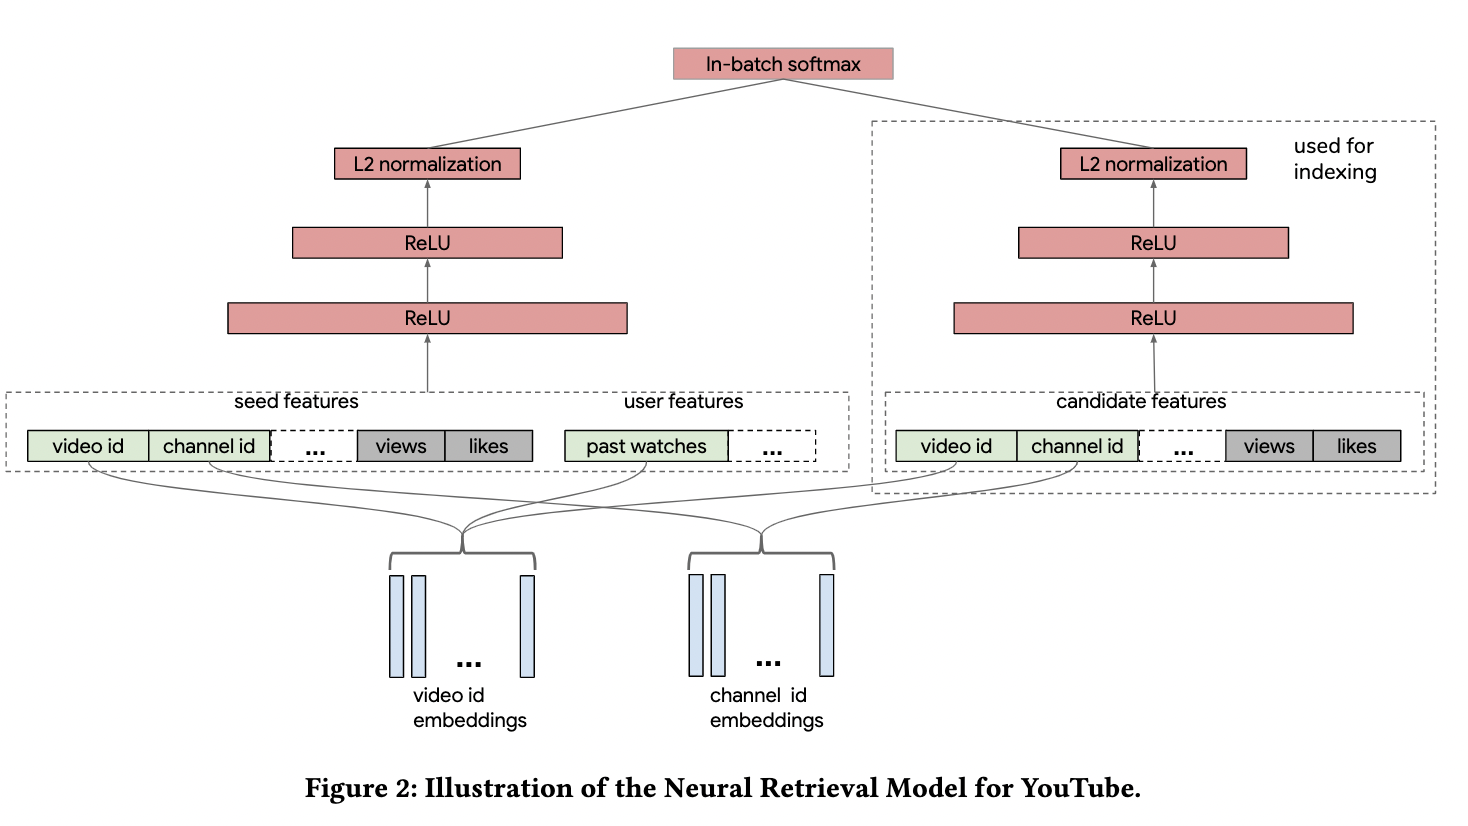
\includegraphics[width=0.9\textwidth]{assets/two_tower.png}
    \caption[Two-Tower Neural Retrieval Model for YouTube]{Two-Tower Neural Retrieval Model for YouTube \cite{YoutubeTwoTower}}
    \label{fig: TwoTowerModel}
\end{figure}

The output of the two-tower model is a vector representing the similarity between item embedding and user embedding, 
it indicates the user's level of interest in the specified item.


\subsubsection{Approximate Nearest Neighbor}

One popular approach to retrieval uses embedding models. 
These models create a dense vector space where users and items are represented as points.
ANN search,
which identifies items closest to the user's representation in the space, 
indicating potential relevance and making them strong candidates for recommendation. figure \ref{fig:Ann} illustrates the concept of ANN search

\begin{figure}[H]
    \centering
    \includegraphics[width=0.9\textwidth]{assets/Approximate Nearest Neighbor.jpg}
    \caption[Approximate Nearest Neighbor]{Approximate Nearest Neighbor}
    \label{fig:Ann}
\end{figure}



\subsection{Filtering Stage}

After retrieving a set of candidate items, the next stage is filtering them according to business rules and constraints.
This stage ensures that only valid candidates are passed to the scoring stage.
For example, products that are out of stock, or products that users already bought.

One possible approach to filtering is using a Bloom filter, which is a space-efficient probabilistic data structure that is used to test whether an element is a member of a set.

Another simpler approach is to use a rule-based system, where the system applies a set of rules to the candidate items to filter out the invalid ones, but it might be less performant than the Bloom filter.


\subsection{Scoring Stage}
% Valid candidates are scored using a richer set of user, item, and session features and a more expressive model such as a deep neural network.

In the scoring stage, valid candidates are scored based on their relevance to the user. Precision in this stage is crucial, more features including user, item, and session features are added that wouldn't have been possibly added in the retrieval stage due to the computational and latency constraints since the retrieval stage processes a large number of items. Moreover, a more expressive model can be used in this stage such as DNN \cite{eugeneyan}. 

Ranking items can be expressed as either a classification problem or a dedicated learning-to-rank problem. In deep learning applications, the final output layer either employs a softmax function to generate preference scores for a set of items or utilizes a sigmoid function to estimate the probability of user interaction (such as clicking or purchasing) for each possible user-item combination \cite{eugeneyan}. 

\subsection{Ordering Stage}
In the ordering stage, We narrow down the choices to the best K options, then adjust their order based on specific business needs. For instance, a product category or manufacturer promotion might influence their ranking \cite{NvidiaRecSysBestPractices}.
